\section{Model Description}

\subsection{Introduction}

This module is modeling a VSCMG connected to a rigid body hub. The VSCMG model has three modes that can be ran: balanced wheels, simple jitter, and fully-coupled imbalanced wheels.

The balanced wheels option is modeling the VSCMG as having their principle inertia axes aligned with spin axis, $\hat{\bm g}_s$, and the center of mass of the wheel is coincident with $\hat{\bm g}_s$. This results in the VSCMG not changing the mass properties of the spacecraft and results in simpler equations. The simple jitter option is approximating the jitter due to mass imbalances by applying an external force and torque to the spacecraft that is proportional to the wheel speeds squared. This is an approximation because in reality this is an internal force and torque. Finally, the fully-coupled mode is modeling VSCMG imbalance dynamics by modeling the static and dynamic imbalances as internal forces and torques which is physically realistic and allows for energy and momentum conservation.

Figure \ref{fig:scplusVSCMG} shows the frame and variable definitions used for this problem. The formulation involves a rigid hub with its center of mass location labeled as point $B_c$, VSCMGs made of a gimbal and wheel whose center of mass locations are labeled as $G_{c_i}$ and  $W_{c_i}$ respectively. The frames being used for this formulation are the body-fixed frame, \frameDefinition{B}, the gimbal frame of the $i^\text{th}$ gimbal, $\mathcal{G}_i:\{\hat{\bm g}_{s_i},\hat{\bm g}_{t_i},\hat{\bm g}_{g_i}\}$ which is also body-fixed, and the wheel-fixed frame of the $i^\text{th}$ RW, $\mathcal{W}_i:\{\hat{\bm g}_{s_i},\hat{\bm w}_{2_i},\hat{\bm w}_{3_i}\}$. The dynamics are modeled with respect to the $\mathcal{B}$ frame which can be generally oriented. The $\mathcal{W}_i$ frame is oriented such that the $\hat{\bm g}_{s_i}$ axis is aligned with the RW spin axis  which is the same as the gimbal torque axis $\hat{\bm g}_{s_{i}}$, the $\hat{\bm w}_{2_i}$ axis is perpendicular to $\hat{\bm g}_{s_i}$ and points in the direction towards the RW center of mass $W_{c_i}$. The $\hat{\bm w}_{3_i}$ completes the right hand rule. The $\mathcal{M}_i$ frame is defined as being equal to the $\mathcal{W}_i$ frame at the beginning of the simulation and therefore the $\mathcal{W}_i$ and $\mathcal{G}_i$ frames are offset by an angle, $\theta_i$, about the $\hat{\bm g}_{s_i} = \hat{\bm g}_{s_i}$ axes.
	
A few more key variables in Figure~\ref{fig:scplusVSCMG} need to be defined. The rigid spacecraft structure without the VSCMGs is called the hub.  Point $B$ is the origin of the $\mathcal{B}$ frame and is a general body-fixed point that does not have to be identical to the total spacecraft center of mass, nor the rigid hub center of mass $B_{c}$. Point $W_i$ is the origin of the $\mathcal{W}_i$ frame and can also have any location relative to point $B$. Point $C$ is the center of mass of the total spacecraft system including the rigid hub and the VSCMGs. Due to the VSCMG imbalance, the vector $\bm c$, which points from point $B$ to point $C$, will vary as seen by a body-fixed observer. The scalar variable $d_i$ is the center of mass offset of the VSCMG, or the distance from the spin axis, $\hat{\bm g}_{\text{s}_i}$ to $W_{c_i}$.  

The key equations used to model the dynamics of VSCMGs are produced in a form to make use of back-substitution, a computationally efficent way to solve rigid body dynamics. An explaination of backsubstitution and the corresponding equations are highlighted below. For a more thorough explaination of back-substitution and the derivation of the equations of motion can be found in  \href{http://hanspeterschaub.info/Papers/grads/JohnAlcorn.pdf}{Alcorn 2017}\cite{alcorn2017}.

\begin{figure}[htbp]
	\centerline{
		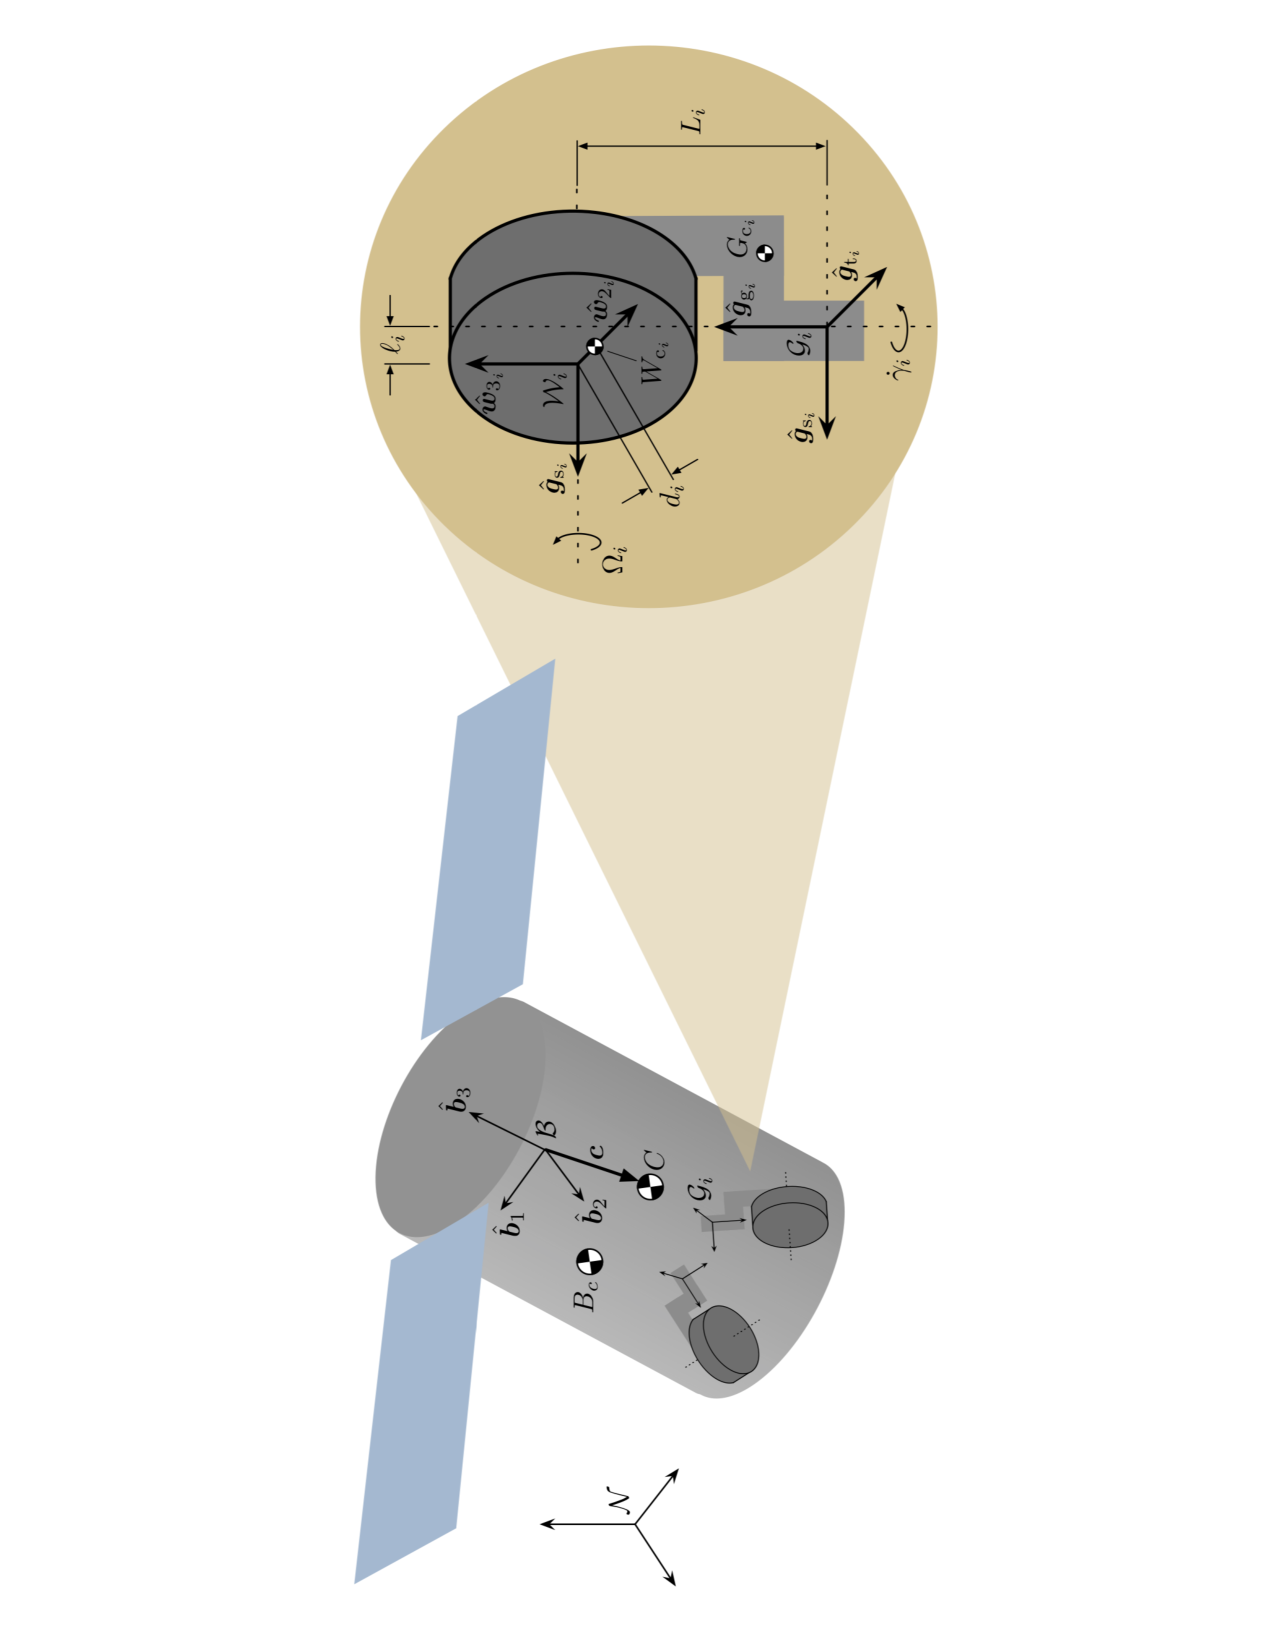
\includegraphics[angle=-90,width=0.8\textwidth]{Figures/scplusVSCMG}}
	\caption{VSCMG and spacecraft frame and variable definitions}
	\label{fig:scplusVSCMG}
\end{figure}

\subsection{Back-Substitution}
The goal of back-substitution is to manipulate the rotational and translational equations of motion to conform to the following form,
\begin{equation}
\begin{bmatrix}
[A] & [B]\\
[C] & [D]
\end{bmatrix} \begin{bmatrix}
\ddot{\bm r}_{B/N}\\
\dot{\bm\omega}_{\cal B/N}
\end{bmatrix} = \begin{bmatrix}
\bm v_{\text{trans}}\\
\bm v_{\text{rot}}
\end{bmatrix}
\label{eq:backsub}
\end{equation}
where $[A]$, $[B]$, $[C]$, and $[D]$ are 3x3 matrices representing $\ddot{\bm r}_{B/N}$ and $\dot{\bm\omega}_{\cal B/N}$ coefficients within the translational and rotational EOMs. $\bm v_{\text{trans}}$ is a 3x1 vector that represents the right-hand side (RHS) of the translational EOM, and $\bm v_{\text{rot}}$ is a 3x1 vector that represents the RHS of the rotational EOM. The matrices $[A]$, $[B]$, $[C]$, $[D]$ and vectors $\bm v_{\text{trans}}$, $\bm v_{\text{rot}}$ are broken down as follows.
\begin{gather}
[A] = [A_\text{hub}] + [A_\text{contr}]
\\
[B] = [B_\text{hub}] + [B_\text{contr}]
\\
[C] = [C_\text{hub}] + [C_\text{contr}]
\\
[D] = [D_\text{hub}] + [D_\text{contr}]
\\
\bm v_{\text{trans}} = \bm v_{\text{trans,hub}} + \bm v_{\text{trans,contr}}
\\
\bm v_{\text{rot}} = \bm v_{\text{rot,hub}} + \bm v_{\text{rot,contr}}
\end{gather}
where $[A_\text{hub}]$ represents the contribution to $[A]$ from the spacecraft hub and $[A_\text{contr}]$ represents the contribution to $[A]$ from the effectors (i.e. RWs or VSCMGs), etc. $[A_\text{hub}]$ etc are the same regardless of the type of effector used, and are provided in the equation below.
\begin{gather}
[A_\text{hub}] = m_{\text{sc}}[I_{3\times3}]
\\
[B_\text{hub}] = -m_{\text{sc}}[\tilde{\bm{c}}]
\\
[C_\text{hub}] = m_{\text{\text{sc}}}[\tilde{\bm{c}}]
\\
[D_\text{hub}] = [I_{\text{sc},B}]
\\
\bm v_{\text{trans,hub}} = \bm{F} - 2m_{\text{sc}}[\tilde{\bm{\omega}}]\bm{c}' - m_{\text{sc}}[\tilde{\bm{\omega}}]^2\bm{c}
\\
\bm v_{\text{rot,hub}} = \bm{L}_B - [I_{\text{sc},B}]'\bm{\omega} - [\tilde{\bm\omega}][I_{\text{sc},B}]\bm\omega
\end{gather}

\subsection{Balanced VSCMG}
\subsubsection{Equations of Motion}
The balanced VSCMG equations of motion are provided here for the reader's convenience. Note that translation is not coupled with $\dot{\Omega}$ or $\ddot{\gamma}_i$.
\begin{equation}\label{eq:vscmgTranslationSimpleBS_BACKSUBAPP}
m_\text{sc}\ddot{\bm r}_{B/N} - m_\text{sc}[\tilde{\bm{c}}]\dot{\bm \omega} 
= \bm{F} - 2m_\text{sc}[\tilde{\bm{\omega}}]\bm{c}' - m_\text{sc}[\tilde{\bm{\omega}}]^2\bm{c} 
\end{equation}
The rotational equation of motion includes $\dot{\Omega}_i$ and $\ddot{\gamma}_i$ terms, and is thus coupled with VSCMG motion as seen below.
\begin{multline}
m_{\text{\text{sc}}}[\tilde{\bm{c}}]\ddot{\bm r}_{B/N} + [I_{\text{sc},B}]\dot{\bm\omega}
+\sum\limits_{i=1}^{N}I_{\text{V}_{g_i}}\hat{\bm{g}}_{\text{g}_i} \ddot{\gamma}_i
+\sum\limits_{i=1}^{N}I_{\text{W}_{s_i}}\hat{\bm{g}}_{\text{s}_i} \dot{\Omega}_i
\\
= \bm{L}_B - [I_{\text{sc},B}]'\bm{\omega} - [\tilde{\bm\omega}][I_{\text{sc},B}]\bm\omega
-\sum\limits_{i=1}^{N} \Big[ 
+ I_{\text{W}_{t_i}}\Omega\dot{\gamma}\hat{\bm{g}}_{\text{t}_i} + \Omega_i\dot{\gamma}_i(I_{\text{W}_{s_i}}-I_{\text{W}_{t_i}})\hat{\bm{g}}_{\text{t}_i} \\+ [\tilde{\bm\omega}][I_{\text{G}_i,G_{c_i}}]\dot{\gamma}_i\hat{\bm{g}}_{\text{g}_i} + [\tilde{\bm{\omega}}][I_{\text{W}_i,W_{c_i}}]\bm{\omega}_{\mathcal{W}_i/\cal B}
\Big]
\label{eq:vscmgRotationSimpleBS_BACKSUBAPP}
\end{multline}
The gimbal torque equation is given below.
\begin{equation}
I_{\text{V}_{g_i}}(\hat{\bm g}_{\text{g}_i}^T\dot{\bm{\omega}}
+  \ddot{\gamma}_i)
= u_{\text{g}_i} + (I_{\text{V}_{s_i}}-I_{\text{V}_{t_i}})\omega_s\omega_t + I_{\text{W}_{s_i}}\Omega_i\omega_t
\label{eq:vscmgGimbalTorqueSimpleBS_BACKSUBAPP}
\end{equation}
The wheel torque equation is given below.
\begin{equation}
I_{\text{W}_{s_i}}(\hat{\bm g}_{\text{s}_i}^T\dot{\bm\omega} + \dot{\Omega}_i)
=-I_{\text{W}_{s_i}}\omega_t\dot{\gamma}_i + u_{\text{s}_i}
\label{eq:vscmgWheelTorqueSimpleBS_BACKSUBAPP}
\end{equation} 

\subsubsection{Modified EOM for Back-Substitution}
To make use of back-substitution and define the back-substitution contribution matrices for a balanced VSCMG, the EOM must be arranged into the following form:
\begin{multline}
m_{\text{\text{sc}}}[\tilde{\bm{c}}]\ddot{\bm r}_{B/N} + \Big[ [I_{\text{sc},B}] - \sum\limits_{i=1}^{N}\big(I_{\text{V}_{g_i}}\hat{\bm{g}}_{\text{g}_i}\hat{\bm g}_{\text{g}_i}^T\dot{\bm{\omega}} + I_{\text{W}_{s_i}}\hat{\bm{g}}_{\text{s}_i}\hat{\bm g}_{\text{s}_i}^T\big)\Big]\dot{\bm\omega}
\\
= \bm{L}_B - [I_{\text{sc},B}]'\bm{\omega} - [\tilde{\bm\omega}][I_{\text{sc},B}]\bm\omega
-\sum\limits_{i=1}^{N} \Big[ 
\big( u_{\text{s}_i}-I_{\text{W}_{s_i}}\omega_t\dot{\gamma}_i \big) \hat{\bm{g}}_{\text{s}_i} + I_{\text{W}_{s_i}}\Omega\dot{\gamma}\hat{\bm{g}}_{\text{t}_i} \\+\big( u_{\text{g}_i} + (I_{\text{V}_{s_i}}-I_{\text{V}_{t_i}})\omega_s\omega_t + I_{\text{W}_{s_i}}\Omega_i\omega_t\big)\hat{\bm{g}}_{\text{g}_i}+ [\tilde{\bm\omega}][I_{\text{G}_i,G_{c_i}}]\dot{\gamma}_i\hat{\bm{g}}_{\text{g}_i} + [\tilde{\bm{\omega}}][I_{\text{W}_i,W_{c_i}}]\bm{\omega}_{\mathcal{W}_i/\cal B}
\Big]
\label{eq:vscmgRotationSimpleBS2_BACKSUBAPP}
\end{multline}

\subsubsection{Back-Substitution Contribution Matrices}
The balanced VSCMG back-substitution contribution matrices are given by,
\begin{gather}
[A_\text{contr}] = [0_{3 \times 3}]
\\
[B_\text{contr}] = [0_{3 \times 3}]
\\
[C_\text{contr}] = [0_{3 \times 3}]
\\
[D_\text{contr}] = - \sum\limits_{i=1}^{N}\big[I_{\text{V}_{g_i}}\hat{\bm{g}}_{\text{g}_i}\hat{\bm g}_{\text{g}_i}^T + I_{\text{W}_{s_i}}\hat{\bm{g}}_{\text{s}_i}\hat{\bm g}_{\text{s}_i}^T\big]
\\
\bm v_{\text{trans,contr}} = \bm 0
\end{gather}
\begin{multline}
\bm v_{\text{rot,contr}} =  -\sum\limits_{i=1}^{N} \Big[ 
\big( u_{\text{s}_i}-I_{\text{W}_{s_i}}\omega_t\dot{\gamma}_i \big) \hat{\bm{g}}_{\text{s}_i} + I_{\text{W}_{s_i}}\Omega\dot{\gamma}\hat{\bm{g}}_{\text{t}_i} +\big( u_{\text{g}_i} + (I_{\text{V}_{s_i}}-I_{\text{V}_{t_i}})\omega_s\omega_t + I_{\text{W}_{s_i}}\Omega_i\omega_t\big)\hat{\bm{g}}_{\text{g}_i}\\+ [\tilde{\bm\omega}][I_{\text{G}_i,G_{c_i}}]\dot{\gamma}_i\hat{\bm{g}}_{\text{g}_i} + [\tilde{\bm{\omega}}][I_{\text{W}_i,W_{c_i}}]\bm{\omega}_{\mathcal{W}_i/\cal B}
\Big]
\end{multline}

\subsection{Imbalanced VSCMG}

\subsubsection{Translational EOMs}
The translational equation of motion for an imbalanced VSCMG is:
\begin{multline}
\ddot{\bm r}_{B/N} - [\tilde{\bm{c}}]\dot{\bm \omega} 
+ \frac{1}{m_{\text{sc}}} \sum\limits_{i=1}^{N} \left[ m_{\text{G}_i} \left[\tilde{\hat{\bm g}}_{\text{g}_i} \right] \bm{r}_{G_{c_i}/G_i} - m_{\text{W}_i}d_ic\theta_i\hat{\bm{g}}_{\text{s}_i} + m_{\text{W}_i}\ell_i\hat{\bm{g}}_{\text{t}_i} \right] \ddot{\gamma}_i
+ \frac{1}{m_{\text{sc}}} \sum\limits_{i=1}^{N} \left[ m_{\text{W}_i}d_i\hat{\bm w}_{3_i} \right] \dot{\Omega}_i
\\= \ddot{\bm r}_{C/N} - 2[\tilde{\bm{\omega}}]\bm{c}' - [\tilde{\bm{\omega}}][\tilde{\bm{\omega}}]\bm{c} 
- \frac{1}{m_{\text{sc}}} \sum\limits_{i=1}^{N} \Big[ 
m_{\text{G}_i}\dot{\gamma}_i[\tilde{\hat{\bm g}}_{\text{g}_i}] \bm{r}_{G_{c_i}/B}'
\\+ m_{\text{W}_i} \big[ \left(2d_i\dot{\gamma}_i\Omega_i\text{s}\theta_i - \ell_i\dot{\gamma}_i^2 \right)\hat{\bm{g}}_{\text{s}_i} - d_i\dot{\gamma}_i^2c\theta_i\hat{\bm{g}}_{\text{t}_i} - d_i\Omega_i^2 \hat{\bm{w}}_{2_i} \big] \Big]
\end{multline}
This equation represents 3 DOF and contains all second order states ($\ddot{\bm r}_{B/N}$, $\dot{\bm \omega}$, $\ddot{\gamma}_i$, $\dot{\Omega}_i$). Removing wheel imbalance terms and assuming a symmetrical VSCMG (i.e. $\bm{r}_{G_{c_i}/G_i} = \bm{0}$, $\ell_i = 0$, $d_i = 0$) gives the following balanced VSCMG transational equation of motion.
\begin{equation}
	m_\text{sc}\ddot{\bm r}_{B/N} - m_\text{sc}[\tilde{\bm{c}}]\dot{\bm \omega} 
	= \bm{F} - 2m_\text{sc}[\tilde{\bm{\omega}}]\bm{c}' - m_\text{sc}[\tilde{\bm{\omega}}]^2\bm{c} 
	\label{eq:vscmgTranslationSimple}
\end{equation}

Thus, the balanced VSCMG translational equation of motion does not contain any second-order terms relating to the wheel or gimbal, and agrees with Eq. \ref{eq:vscmgTranslationSimpleBS_BACKSUBAPP}.

\subsubsection{Rotational EOMs}

The rotational equations of motion are:
\begin{equation}
	\begin{split}
		m_{\text{\text{sc}}}[\tilde{\bm{c}}]\ddot{\bm r}&_{B/N} + [I_{\text{sc},B}]\dot{\bm\omega}
		+\sum\limits_{i=1}^{N} \Big[ [I_{\text{G}_i,G_{c_i}}]\hat{\bm{g}}_{\text{g}_i} + m_{\text{G}_i}[\tilde{\bm{r}}_{G_{c_i}/B}][\tilde{\hat{\bm g}}_{\text{g}_i}]\bm{r}_{G_{c_i}/G_i} + [I_{\text{W}_i,W_{c_i}}]\hat{\bm{g}}_{\text{g}_i} 
		\\
		+ m_{\text{W}_i}&[\tilde{\bm{r}}_{W_{c_i}/B}]( \ell_i\hat{\bm{g}}_{\text{t}_i} - d_ic\theta_i\hat{\bm{g}}_{\text{s}_i}) \Big] \ddot{\gamma}_i
		+\sum\limits_{i=1}^{N} \left[ [I_{\text{W}_i,W_{c_i}}]\hat{\bm{g}}_{\text{s}_i} + m_{\text{W}_i}d_i[\tilde{\bm{r}}_{W_{c_i}/B}]\hat{\bm w}_{3_i} \right] \dot{\Omega}_i
		\\
		=& \bm{L}_B - [I_{\text{sc},B}]'\bm{\omega} - [\tilde{\bm\omega}][I_{\text{sc},B}]\bm\omega
		-\sum\limits_{i=1}^{N} \Big[ 
		[I_{\text{G}_i,G_{c_i}}]'\dot{\gamma}_i\hat{\bm{g}}_{\text{g}_i} + [\tilde{\bm\omega}][I_{\text{G}_i,G_{c_i}}]\dot{\gamma}_i\hat{\bm{g}}_{\text{g}_i} + m_{\text{G}_i}[\tilde{\bm{\omega}}][\tilde{\bm{r}}_{G_{c_i}/B}]\bm{r}'_{G_{c_i}/B}
		\\&+ m_{\text{G}_i}\dot{\gamma}_i[\tilde{\bm{r}}_{G_{c_i}/B}][\tilde{\hat{\bm g}}_{\text{g}_i}]\bm{r}'_{G_{c_i}/G_i}
		+ [I_{\text{W}_i,W_{c_i}}]\Omega\dot{\gamma}\hat{\bm{g}}_{\text{t}_i} + [I_{\text{W}_i,W_{c_i}}]'\bm{\omega}_{\mathcal{W}_i/\cal B} + [\tilde{\bm{\omega}}][I_{\text{W}_i,W_{c_i}}]\bm{\omega}_{\mathcal{W}_i/\cal B} 
		\\
		&+ m_{\text{W}_i}[\tilde{\bm{\omega}}][\tilde{\bm{r}}_{W_{c_i}/B}]\bm{r}'_{W_{c_i}/B} + m_{\text{W}_i}[\tilde{\bm{r}}_{W_{c_i}/B}]\left[\left(2d_i\dot{\gamma}_i\Omega_i\text{s}\theta_i - \ell_i\dot{\gamma}_i^2\right)\hat{\bm{g}}_{\text{s}_i} - d_i\dot{\gamma}_i^2c\theta_i\hat{\bm{g}}_{\text{t}_i} - d_i\Omega_i^2 \hat{\bm{w}}_{2_i} \right]
		\Big]
	\end{split}
\label{eq:rotation}
\end{equation}
The rotational equation of motion for a VSCMG with balanced wheels may be found by setting imbalance terms to zero, leading to:
\begin{multline}
m_{\text{\text{sc}}}[\tilde{\bm{c}}]\ddot{\bm r}_{B/N} + [I_{\text{sc},B}]\dot{\bm\omega}
+\sum\limits_{i=1}^{N}I_{\text{V}_{g_i}}\hat{\bm{g}}_{\text{g}_i} \ddot{\gamma}_i
+\sum\limits_{i=1}^{N}I_{\text{W}_{s_i}}\hat{\bm{g}}_{\text{s}_i} \dot{\Omega}_i
\\
= \bm{L}_B - [\tilde{\bm\omega}][I_{\text{sc},B}]\bm\omega
-\sum\limits_{i=1}^{N} \Big[ 
\omega_t\dot{\gamma}_i(I_{\text{V}_{s_i}}-I_{\text{V}_{t_i}}+I_{\text{V}_{g_i}}) \hat{\bm{g}}_{\text{s}_i}
\\+ \big[ \omega_s\dot{\gamma}_i(I_{\text{V}_{s_i}}-I_{\text{V}_{t_i}}-I_{\text{V}_{g_i}}) + I_{\text{W}_{s_i}}\Omega_i(\dot{\gamma} + \omega_g) \big]\hat{\bm{g}}_{\text{t}_i}
-\omega_tI_{\text{W}_{s_i}}\Omega_i\hat{\bm{g}}_{\text{g}_i} \Big]
\label{eq:vscmgRotationSimple}
\end{multline}
This equation agrees with that found in Eq.  \ref{eq:vscmgRotationSimpleBS_BACKSUBAPP}. 

\subsubsection{Gimbal Torque Equation}
The VSCMG gimbal torque equation of motion is given by:
\begin{multline}
\hat{\bm g}_{\text{g}_i}^T \Bigg[ m_{\text{V}_i}[\tilde{\bm r}_{V_{c_i}/G_i}] \Bigg] \ddot{\bm r}_{B/N}
+ \hat{\bm g}_{\text{g}_i}^T \Bigg[ [I_{\text{V}_i,V_{c_i}}] + m_{\text{V}_i}[\tilde{\bm r}_{V_{c_i}/G_i}][\tilde{\bm{r}}_{V_{c_i}/B}]^T \Bigg] \dot{\bm{\omega}}
+ \hat{\bm g}_{\text{g}_i}^T \Bigg[ [I_{\text{G}_i,G_{c_i}}]\hat{\bm{g}}_{\text{g}_i} 
\\+ [I_{\text{W}_i,W_{c_i}}]\hat{\bm{g}}_{\text{g}_i} + [P_i] \big(\ell_i\hat{\bm{g}}_{\text{t}_i} - d_ic\theta_i\hat{\bm{g}}_{\text{s}_i}\big) + [Q_i] [\tilde{\hat{\bm g}}_{\text{g}_i}]\bm{r}_{G_{c_i}/G_i} \Bigg] \ddot{\gamma}_i
+ \hat{\bm g}_{\text{g}_i}^T \Bigg[ [I_{\text{W}_i,W_{c_i}}]\hat{\bm{g}}_{\text{s}_i} + [P_i] d_i\hat{\bm w}_{3_i} \Bigg] \dot{\Omega}_i
\\ = - \hat{\bm g}_{\text{g}_i}^T \Bigg[ \dot{\gamma}_i[Q_i][\tilde{\hat{\bm g}}_{\text{g}_i}]\bm{r}'_{G_{c_i}/G_i} + [P_i] \big[\left(2d_i\dot{\gamma}_i\Omega_i\text{s}\theta_i - \ell_i\dot{\gamma}_i^2\right)\hat{\bm{g}}_{\text{s}_i} - d_i\dot{\gamma}_i^2c\theta_i\hat{\bm{g}}_{\text{t}_i} - d_i\Omega_i^2 \hat{\bm{w}}_{2_i}\big]
\\+[I_{\text{G}_i,G_{c_i}}]'\bm\omega_{\mathcal{G}_i/\cal N} + [\tilde{\bm\omega}][I_{\text{G}_i,G_{c_i}}]\bm\omega_{\mathcal{G}_i/\cal N} + [I_{\text{W}_i,W_{c_i}}]\Omega\dot{\gamma}\hat{\bm{g}}_{\text{t}_i} + [I_{\text{W}_i,W_{c_i}}]'\bm\omega_{\mathcal{W}_i/\cal N} \\+ [\tilde{\bm{\omega}}][I_{\text{W}_i,W_{c_i}}]\bm\omega_{\mathcal{W}_i/\cal N}
+ m_{\text{G}_i}[\tilde{\bm{r}}_{G_{c_i}/V_{c_i}}] \big( 2[\tilde{\bm\omega}]\bm{r}'_{G_{c_i}/V_{c_i}} + [\tilde{\bm\omega}]^2\bm{r}_{G_{c_i}/V_{c_i}}\big)
\\ + m_{\text{W}_i}[\tilde{\bm{r}}_{W_{c_i}/V_{c_i}}]\big( 2[\tilde{\bm\omega}]\bm{r}'_{W_{c_i}/V_{c_i}} + [\tilde{\bm\omega}]^2\bm{r}_{W_{c_i}/V_{c_i}}\big)
+ m_{\text{V}_i}[\tilde{\bm r}_{V_{c_i}/G_i}]\big( 2[\tilde{\bm\omega}]\bm{r}'_{V_{c_i}/B} + [\tilde{\bm\omega}]^2\bm{r}_{V_{c_i}/B} \big) \Bigg] + u_{\text{g}_i}
\label{eq:vscmgtorque}
\end{multline} 
Where,
\begin{gather}
[I_{\text{V}_i,V_{c_i}}] = [I_{\text{G}_i,V_{c_i}}] + [I_{\text{W}_i,V_{c_i}}]
\\
[I_{\text{G}_i,V_{c_i}}] = [I_{\text{G}_i,G_{c_i}}] + m_{\text{G}_i}[\tilde{\bm{r}}_{G_{c_i}/V_{c_i}}][\tilde{\bm{r}}_{G_{c_i}/V_{c_i}}]^T
\\
[I_{\text{W}_i,V_{c_i}}] = [I_{\text{W}_i,W_{c_i}}] + m_{\text{W}_i}[\tilde{\bm{r}}_{W_{c_i}/V_{c_i}}][\tilde{\bm{r}}_{W_{c_i}/V_{c_i}}]^T
\\
[P_i] = m_{\text{W}_i}\rho_{G_i}[\tilde{\bm{r}}_{W_{c_i}/V_{c_i}}] - m_{\text{G}_i}\rho_{W_i}[\tilde{\bm{r}}_{G_{c_i}/V_{c_i}}] + m_{\text{W}_i}[\tilde{\bm r}_{V_{c_i}/G_i}]
\\
[Q_i] = m_{\text{G}_i}\rho_{W_i}[\tilde{\bm{r}}_{G_{c_i}/V_{c_i}}] - m_{\text{W}_i}\rho_{G_i}[\tilde{\bm{r}}_{W_{c_i}/V_{c_i}}] + m_{\text{G}_i}[\tilde{\bm r}_{V_{c_i}/G_i}]
\\
[\tilde{\bm\omega}]^2 = [\tilde{\bm\omega}][\tilde{\bm\omega}]
\end{gather}
Removing all imbalance terms, ~\eqref{eq:vscmgtorque} simplifies to the equation found in \eqref{eq:vscmgGimbalTorqueSimpleBS_BACKSUBAPP}
\begin{equation}
I_{\text{V}_{g_i}}(\hat{\bm g}_{\text{g}_i}^T\dot{\bm{\omega}}
+  \ddot{\gamma}_i)
 = u_{\text{g}_i} + (I_{\text{V}_{s_i}}-I_{\text{V}_{t_i}})\omega_s\omega_t + I_{\text{W}_{s_i}}\Omega_i\omega_t
\label{eq:vscmgGimbalTorqueSimple}
\end{equation}

\subsubsection{Wheel Torque Equation}

The wheel torque equation is given by:
\begin{multline}
		\left[ m_{\text{W}_i}d_i\hat{\bm w}_{3_i}^T \right] \ddot{\bm r}_{B/N} + \left[ \hat{\bm g}_{\text{s}_i}^T[I_{\text{W}_i,W_{c_i}}] + m_{\text{W}_i}d_i\hat{\bm g}_{\text{s}_i}^T[\tilde{\hat{\bm w}}_{2_i}][\tilde{\bm{r}}_{W_{c_i}/B}]^T \right] \dot{\bm\omega}
		\\
		+\left[ J_{12_i}s\theta_i + J_{13_i}c\theta_i - m_{\text{W}_i}d_i\ell_is\theta_i \right] \ddot{\gamma}_i 
		+ \left[ J_{11_i}  + m_{\text{W}_i}d_i^2 \right] \dot{\Omega}_i
		\\
		=-\hat{\bm g}_{\text{s}_i}^T \Bigg[ [I_{\text{W}_i,W_{c_i}}]'\bm\omega_{\mathcal{W}_i/\cal N} + [\tilde{\bm{\omega}}][I_{\text{W}_i,W_{c_i}}]\bm\omega_{\mathcal{W}_i/\cal N}  + m_{\text{W}_i}d_i[\tilde{\hat{\bm w}}_{2_i}] \Big[ 2[\tilde{\bm{r}}'_{W_{c_i}/B}]^T\bm\omega + [\tilde{\bm\omega}][\tilde{\bm\omega}]\bm{r}_{W_{c_i}/B}
		\Big] \Bigg] \\+(J_{13_i}s\theta_i - J_{12_i}c\theta_i)\Omega\dot{\gamma} - m_{\text{W}_i}d_i^2\dot{\gamma}_i^2c\theta_is\theta_i
		+ u_{\text{s}_i}
\end{multline}  
Removing imbalance terms gives (recall that for the simplified case $\theta_i = 0$),
\begin{equation}
	I_{\text{W}_{s_i}}(\hat{\bm g}_{\text{s}_i}^T\dot{\bm\omega} + \dot{\Omega}_i)
	=-I_{\text{W}_{s_i}}\omega_t\dot{\gamma}_i + u_{\text{s}_i}
\end{equation} 
which agrees with \eqref{eq:vscmgWheelTorqueSimpleBS_BACKSUBAPP}.

\subsubsection{Modified EOM for Back-Substitution}

\subparagraph{Translational EOM}

This aforementioned translation equation of motion may be rewritten to confirm with back-substitution requirements in the following way:
\begin{equation}
\ddot{\bm r}_{B/N} - [\tilde{\bm{c}}]\dot{\bm \omega} + \frac{1}{m_{\text{sc}}} \sum\limits_{i=1}^{N}\bm{u}_{r_i}\ddot{\gamma}_i + \frac{1}{m_{\text{sc}}} \sum\limits_{i=1}^{N}\bm{v}_{r_i}\dot{\Omega}_i = \ddot{\bm r}_{C/N} - 2[\tilde{\bm{\omega}}]\bm{c}' - [\tilde{\bm{\omega}}]^2\bm{c} - \frac{1}{m_{\text{sc}}} \sum\limits_{i=1}^{N}\bm{k}_{r_i}
\label{eq:transabbr}
\end{equation}
where,
\begin{align}
\bm{u}_{r_i} &= m_{\text{G}_i}[\tilde{\hat{\bm g}}_{\text{g}_i}] \bm{r}_{G_{c_i}/G_i} - m_{\text{W}_i}d_ic\theta_i\hat{\bm{g}}_{\text{s}_i} + m_{\text{W}_i}\ell_i\hat{\bm{g}}_{\text{t}_i}
\\
\bm{v}_{r_i} &= m_{\text{W}_i}d_i\hat{\bm w}_{3_i}
\\
\bm{k}_{r_i} &= m_{\text{G}_i}\dot{\gamma}_i[\tilde{\hat{\bm g}}_{\text{g}_i}] \bm{r}_{G_{c_i}/B}'
+ m_{\text{W}_i} \left[ \left(2d_i\dot{\gamma}_i\Omega_i\text{s}\theta_i - \ell_i\dot{\gamma}_i^2\right)\hat{\bm{g}}_{\text{s}_i} - d_i\dot{\gamma}_i^2c\theta_i\hat{\bm{g}}_{\text{t}_i} - d_i\Omega_i^2 \hat{\bm{w}}_{2_i} \right]
\end{align}

\begin{gather}
\begin{split}
\Bigg[ m_{\text{sc}}[I_{3\times3}]+ \sum\limits_{i=1}^{N}\Bigg(\bm{u}_{r_i}\bm{a}_{\gamma_i}^T + \frac{\big(\bm{v}_{r_i} + \bm{u}_{r_i}c_{\gamma_i}\big)\big(\bm{a}_{\Omega_i}^T + c_{\Omega_i}\bm{a}_{\gamma_i}^T\big)}{1 - c_{\Omega_i}c_{\gamma_i}}\Bigg) \Bigg] \ddot{\bm r}_{B/N}
\\+ \Bigg[- m_{\text{sc}}[\tilde{\bm{c}}] +  \sum\limits_{i=1}^{N}\Bigg(\bm{u}_{r_i}\bm{b}_{\gamma_i}^T + \frac{\big(\bm{v}_{r_i} + \bm{u}_{r_i}c_{\gamma_i}\big)\big(\bm{b}_{\Omega_i}^T + c_{\Omega_i}\bm{b}_{\gamma_i}^T\big)}{1 - c_{\Omega_i}c_{\gamma_i}}\Bigg)\Bigg] \dot{\bm{\omega}}
\\= \bm{F} - 2m_{\text{sc}}[\tilde{\bm{\omega}}]\bm{c}' - m_{\text{sc}}[\tilde{\bm{\omega}}]^2\bm{c} -  \sum\limits_{i=1}^{N}\Bigg(\bm{k}_{r_i}+\bm{u}_{r_i}d_{\gamma_i} + \frac{\big(\bm{v}_{r_i} + \bm{u}_{r_i}c_{\gamma_i}\big)\big(c_{\Omega_i}d_{\gamma_i} + d_{\Omega_i}\big)}{1 - c_{\Omega_i}c_{\gamma_i}}\Bigg)
\end{split}
\end{gather}

\subparagraph{Rotational EOM}

This equation may be abbreviated as,
\begin{equation}
\begin{split}
m_{\text{\text{sc}}}[\tilde{\bm{c}}]\ddot{\bm r}_{B/N} + [I_{\text{sc},B}]\dot{\bm\omega} +  \sum\limits_{i=1}^{N}\bm{u}_{\omega_i}\ddot{\gamma}_i +  \sum\limits_{i=1}^{N}\bm{v}_{\omega_i}\dot{\Omega}_i \\= \bm{L}_B - [I_{\text{sc},B}]'\bm{\omega} - [\tilde{\bm\omega}][I_{\text{sc},B}]\bm\omega - \sum\limits_{i=1}^{N}\bm{k}_{\omega_i}
\end{split}
\label{eq:rotabbr}
\end{equation}
where,
\begin{align}
\begin{split}
\bm{u}_{\omega_i} &=  [I_{\text{G}_i,G_{c_i}}]\hat{\bm{g}}_{\text{g}_i} + m_{\text{G}_i}[\tilde{\bm{r}}_{G_{c_i}/B}][\tilde{\hat{\bm g}}_{\text{g}_i}]\bm{r}_{G_{c_i}/G_i} + [I_{\text{W}_i,W_{c_i}}]\hat{\bm{g}}_{\text{g}_i} + m_{\text{W}_i}[\tilde{\bm{r}}_{W_{c_i}/B}]( \ell_i\hat{\bm{g}}_{\text{t}_i} - d_ic\theta_i\hat{\bm{g}}_{\text{s}_i})
\end{split}
\\
\bm{v}_{\omega_i} &= [I_{\text{W}_i,W_{c_i}}]\hat{\bm{g}}_{\text{s}_i} + m_{\text{W}_i}d_i[\tilde{\bm{r}}_{W_{c_i}/B}]\hat{\bm w}_{3_i}
\\
\begin{split}
\bm{k}_{\omega_i} =  
[I_{\text{G}_i,G_{c_i}}]'\dot{\gamma}_i\hat{\bm{g}}_{\text{g}_i} + [\tilde{\bm\omega}][I_{\text{G}_i,G_{c_i}}]\dot{\gamma}_i\hat{\bm{g}}_{\text{g}_i} + m_{\text{G}_i}[\tilde{\bm{\omega}}][\tilde{\bm{r}}_{G_{c_i}/B}]\bm{r}'_{G_{c_i}/B}
+ m_{\text{G}_i}\dot{\gamma}_i[\tilde{\bm{r}}_{G_{c_i}/B}][\tilde{\hat{\bm g}}_{\text{g}_i}]\bm{r}'_{G_{c_i}/G_i}
\\+ [I_{\text{W}_i,W_{c_i}}]\Omega\dot{\gamma}\hat{\bm{g}}_{\text{t}_i} + [I_{\text{W}_i,W_{c_i}}]'\bm{\omega}_{\mathcal{W}_i/\cal B} + [\tilde{\bm{\omega}}][I_{\text{W}_i,W_{c_i}}]\bm{\omega}_{\mathcal{W}_i/\cal B} + m_{\text{W}_i}[\tilde{\bm{\omega}}][\tilde{\bm{r}}_{W_{c_i}/B}]\bm{r}'_{W_{c_i}/B} \\+ m_{\text{W}_i}[\tilde{\bm{r}}_{W_{c_i}/B}]\left[\left(2d_i\dot{\gamma}_i\Omega_i\text{s}\theta_i - \ell_i\dot{\gamma}_i^2\right)\hat{\bm{g}}_{\text{s}_i} - d_i\dot{\gamma}_i^2c\theta_i\hat{\bm{g}}_{\text{t}_i} - d_i\Omega_i^2 \hat{\bm{w}}_{2_i} \right]
\end{split}
\end{align}

\begin{multline}
\left[ m_{\text{sc}}[\tilde{\bm c}]+ \sum\limits_{i=1}^{N}\Big([I_{\text{rw}_i,W_{c_i}}]\hat{\bm{g}}_{s_i} + m_{\text{rw}_i}d_i[\tilde{\bm{r}}_{W_{c_i}/B}]\hat{\bm{w}}_{3_i}\Big)\bm{a}_{\Omega_i}^T \right] \ddot{\bm r}_{B/N}
\\ 
+ \left[ [I_{\text{sc},B}] + \sum\limits_{i=1}^{N}\Big([I_{\text{rw}_i,W_{c_i}}]\hat{\bm{g}}_{s_i} + m_{\text{rw}_i}d_i[\tilde{\bm{r}}_{W_{c_i}/B}]\hat{\bm{w}}_{3_i}\Big)\bm{b}_{\Omega_i}^T \right] \dot{\bm\omega}_{\cal B/N} 
\\= 
\sum\limits_{i=1}^{N}\Big[ m_{\text{rw}_i}[\tilde{\bm{r}}_{W_{c_i}/B}]d_i \Omega_i^2\hat{\bm{w}}_{2_i}-[I_{\text{rw}_i,W_{c_i}}]'\Omega_i \hat{\bm{g}}_{s_i} -[\tilde{\bm\omega}_{\cal B/N}]\Big([I_{\text{rw}_i,W_{c_i}}]\Omega_i \hat{\bm{g}}_{s_i}+ m_{\text{rw}_i}[\tilde{\bm{r}}_{W_{c_i}/B}]\bm{r}'_{W_{c_i}/B}\Big) \\ 
-\Big([I_{\text{rw}_i,W_{c_i}}]\hat{\bm{g}}_{s_i} + m_{\text{rw}_i}d_i[\tilde{\bm{r}}_{W_{c_i}/B}]\hat{\bm{w}}_{3_i}\Big)c_{\Omega_i}\Big]
\\  -[\tilde{\bm\omega}_{\cal B/N}][I_{\text{sc},B}]\bm\omega_{\cal B/N}-  [I_{\text{sc},B}]'\bm\omega_{\cal B/N} + \bm{L}_B
\end{multline}

\subparagraph{Gimbal Torque Equation}

The gimbal torque equation is,
\begin{multline}
\hat{\bm g}_{\text{g}_i}^T \Bigg[ m_{\text{V}_i}[\tilde{\bm r}_{V_{c_i}/G_i}] \Bigg] \ddot{\bm r}_{B/N}
+ \hat{\bm g}_{\text{g}_i}^T \Bigg[ [I_{\text{V}_i,V_{c_i}}] + m_{\text{V}_i}[\tilde{\bm r}_{V_{c_i}/G_i}][\tilde{\bm{r}}_{V_{c_i}/B}]^T \Bigg] \dot{\bm{\omega}}
+ \hat{\bm g}_{\text{g}_i}^T \Bigg[ [I_{\text{G}_i,G_{c_i}}]\hat{\bm{g}}_{\text{g}_i} \\+ [I_{\text{W}_i,W_{c_i}}]\hat{\bm{g}}_{\text{g}_i} + [P_i] \big(\ell_i\hat{\bm{g}}_{\text{t}_i} - d_ic\theta_i\hat{\bm{g}}_{\text{s}_i}\big) + [Q_i] [\tilde{\hat{\bm g}}_{\text{g}_i}]\bm{r}_{G_{c_i}/G_i} \Bigg] \ddot{\gamma}_i
+ \hat{\bm g}_{\text{g}_i}^T \Bigg[ [I_{\text{W}_i,W_{c_i}}]\hat{\bm{g}}_{\text{s}_i} + [P_i] d_i\hat{\bm w}_{3_i} \Bigg] \dot{\Omega}_i
\\ = - \hat{\bm g}_{\text{g}_i}^T \Bigg[ \dot{\gamma}_i[Q_i][\tilde{\hat{\bm g}}_{\text{g}_i}]\bm{r}'_{G_{c_i}/G_i} + [P_i] \big[\left(2d_i\dot{\gamma}_i\Omega_i\text{s}\theta_i - \ell_i\dot{\gamma}_i^2\right)\hat{\bm{g}}_{\text{s}_i} - d_i\dot{\gamma}_i^2c\theta_i\hat{\bm{g}}_{\text{t}_i} - d_i\Omega_i^2 \hat{\bm{w}}_{2_i}\big]
\\+[I_{\text{G}_i,G_{c_i}}]'\bm\omega_{\mathcal{G}_i/\cal N} + [\tilde{\bm\omega}][I_{\text{G}_i,G_{c_i}}]\bm\omega_{\mathcal{G}_i/\cal N} + [I_{\text{W}_i,W_{c_i}}]\Omega\dot{\gamma}\hat{\bm{g}}_{\text{t}_i} + [I_{\text{W}_i,W_{c_i}}]'\bm\omega_{\mathcal{W}_i/\cal N} \\+ [\tilde{\bm{\omega}}][I_{\text{W}_i,W_{c_i}}]\bm\omega_{\mathcal{W}_i/\cal N}
+ m_{\text{G}_i}[\tilde{\bm{r}}_{G_{c_i}/V_{c_i}}] \big( 2[\tilde{\bm\omega}]\bm{r}'_{G_{c_i}/V_{c_i}} + [\tilde{\bm\omega}]^2\bm{r}_{G_{c_i}/V_{c_i}}\big)
\\ + m_{\text{W}_i}[\tilde{\bm{r}}_{W_{c_i}/V_{c_i}}]\big( 2[\tilde{\bm\omega}]\bm{r}'_{W_{c_i}/V_{c_i}} + [\tilde{\bm\omega}]^2\bm{r}_{W_{c_i}/V_{c_i}}\big)
+ m_{\text{V}_i}[\tilde{\bm r}_{V_{c_i}/G_i}]\big( 2[\tilde{\bm\omega}]\bm{r}'_{V_{c_i}/B} + [\tilde{\bm\omega}]^2\bm{r}_{V_{c_i}/B} \big) \Bigg] + u_{\text{g}_i}
\label{eq:vscmgtorque}
\end{multline} 
where,
\begin{align}
[I_{\text{V}_i,V_{c_i}}] &= [I_{\text{G}_i,V_{c_i}}] + [I_{\text{W}_i,V_{c_i}}]
\\
[I_{\text{G}_i,V_{c_i}}] &= [I_{\text{G}_i,G_{c_i}}] + m_{\text{G}_i}[\tilde{\bm{r}}_{G_{c_i}/V_{c_i}}][\tilde{\bm{r}}_{G_{c_i}/V_{c_i}}]^T
\\
[I_{\text{W}_i,V_{c_i}}] &= [I_{\text{W}_i,W_{c_i}}] + m_{\text{W}_i}[\tilde{\bm{r}}_{W_{c_i}/V_{c_i}}][\tilde{\bm{r}}_{W_{c_i}/V_{c_i}}]^T
\\
[P_i] &= m_{\text{W}_i}\rho_{G_i}[\tilde{\bm{r}}_{W_{c_i}/V_{c_i}}] - m_{\text{G}_i}\rho_{W_i}[\tilde{\bm{r}}_{G_{c_i}/V_{c_i}}] + m_{\text{W}_i}[\tilde{\bm r}_{V_{c_i}/G_i}]
\\
[Q_i] &= m_{\text{G}_i}\rho_{W_i}[\tilde{\bm{r}}_{G_{c_i}/V_{c_i}}] - m_{\text{W}_i}\rho_{G_i}[\tilde{\bm{r}}_{W_{c_i}/V_{c_i}}] + m_{\text{G}_i}[\tilde{\bm r}_{V_{c_i}/G_i}]
\\
[\tilde{\bm\omega}]^2 &= [\tilde{\bm\omega}][\tilde{\bm\omega}]
\end{align}

\subparagraph{Wheel Torque Equation}

 The wheel torque equation is,
\begin{multline}
\left[ m_{\text{W}_i}d_i\hat{\bm w}_{3_i}^T \right] \ddot{\bm r}_{B/N} + \left[ \hat{\bm g}_{\text{s}_i}^T[I_{\text{W}_i,W_{c_i}}] + m_{\text{W}_i}d_i\hat{\bm g}_{\text{s}_i}^T[\tilde{\hat{\bm w}}_{2_i}][\tilde{\bm{r}}_{W_{c_i}/B}]^T \right] \dot{\bm\omega}
\\
+\left[ J_{12_i}s\theta_i + J_{13_i}c\theta_i - m_{\text{W}_i}d_i\ell_is\theta_i \right] \ddot{\gamma}_i 
+ \left[ J_{11_i}  + m_{\text{W}_i}d_i^2 \right] \dot{\Omega}_i
\\
=-\hat{\bm g}_{\text{s}_i}^T \Bigg[ [I_{\text{W}_i,W_{c_i}}]'\bm\omega_{\mathcal{W}_i/\cal N} + [\tilde{\bm{\omega}}][I_{\text{W}_i,W_{c_i}}]\bm\omega_{\mathcal{W}_i/\cal N}  + m_{\text{W}_i}d_i[\tilde{\hat{\bm w}}_{2_i}] \Big[ 2[\tilde{\bm{r}}'_{W_{c_i}/B}]^T\bm\omega + [\tilde{\bm\omega}][\tilde{\bm\omega}]\bm{r}_{W_{c_i}/B}
\Big] \Bigg] \\+(J_{13_i}s\theta_i - J_{12_i}c\theta_i)\Omega\dot{\gamma} - m_{\text{W}_i}d_i^2\dot{\gamma}_i^2c\theta_is\theta_i
+ u_{\text{s}_i}
\end{multline}  

\subsubsection{Back-Substitution Matrices for Imbalanced VSCMG}


The contributions are,
\begin{gather}
[A_\text{contr}] =  \sum\limits_{i=1}^{N}\Big[\bm{u}_{r_i}\bm{a}_{\gamma_i}^T + \big(\bm{v}_{r_i} + \bm{u}_{r_i}c_{\gamma_i}\big)\bm{p}_i^T\Big]
\\
[B_\text{contr}] =  \sum\limits_{i=1}^{N}\Big[\bm{u}_{r_i}\bm{b}_{\gamma_i}^T + \big(\bm{v}_{r_i} + \bm{u}_{r_i}c_{\gamma_i}\big)\bm{q}_i^T\Big]
\\
[C_\text{contr}] = \sum\limits_{i=1}^{N}\Big[\bm{u}_{\omega_i}\bm{a}_{\gamma_i}^T + \big(\bm{v}_{\omega_i} + \bm{u}_{\omega_i}c_{\gamma_i}\big)\bm{p}_i^T\Big]
\\
[D_\text{contr}] = \sum\limits_{i=1}^{N}\Big[\bm{u}_{\omega_i}\bm{b}_{\gamma_i}^T + \big(\bm{v}_{\omega_i} + \bm{u}_{\omega_i}c_{\gamma_i}\big)\bm{q}_i^T\Big]
\\
\bm{v}_\text{trans,contr} =  -  \sum\limits_{i=1}^{N}\Big[\bm{k}_{r_i}+\bm{u}_{r_i}d_{\gamma_i} + \big(\bm{v}_{r_i} + \bm{u}_{r_i}c_{\gamma_i}\big)s_i\Big]
\\
\bm{v}_\text{rot,contr} = -  \sum\limits_{i=1}^{N}\Big[\bm{k}_{\omega_i} +\bm{u}_{\omega_i}d_{\gamma_i}+ \big(\bm{v}_{\omega_i} + \bm{u}_{\omega_i}c_{\gamma_i}\big)s_i\Big]
\end{gather}



